\section{Beregning av opplagerkrefter}
Det er nødvendig å bestemme kreftene som opptrer i rammens opplager for å kunne dimensjonere resten av systemet.


\begin{figure}[H]
\begin{center}
\leavevmode
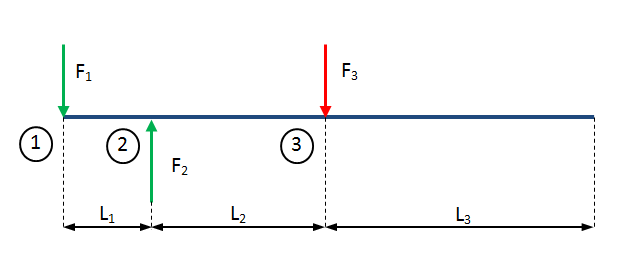
\includegraphics[width=0.8\textwidth]{images/Bilden_1}
\end{center}
\caption{Krefter ramme}
\label{fig:Krefter}
\end{figure}


Kraften $F_3$ tilsvarer halvparten av bilens vekt, siden den blir fordelt på rammens to sider. I denne rapporten er det beregnet med en vekt på bilen tilsvarende 100 kg. Det er videre antatt at denne kraften virker midt på rammen (bilens tyngdepunkt på midten). Rammens egenvekt er neglisjert. \\



Setter opp momentlikevekt om Punkt 1:

\begin{equation}
\sum{M_1}=0
\end{equation}

\begin{equation}
F_3(L_1+L_2)-F_2*L_1=0
\end{equation}
 
\begin{equation}
F_2=\frac{F_3(L_1+L_2)}{L_1}
\end{equation}

\begin{equation}
F_2=\frac{F_3(L_1+L_2)}{L_1}
\end{equation}\\\\

Setter opp kraftlikevekt i Y-retning:


\begin{equation}
\sum{F_Y}=0
\end{equation}

\begin{equation}
F_2-F_1-F_3=0
\end{equation}

\begin{equation}
F_2-F_1-F_3=0
\end{equation}
 
\begin{equation}
F_1=F_2-F_3
\end{equation}


\begin{equation}
F_1=\frac{F_3(L_1+L_2)}{L_1}-F_3
\end{equation} \\

Lager en graf for å se forholdet mellom $L_1$ og opplagerkreftene $F_1$ og $F_2$:

\begin{figure}[H]
\begin{center}
\leavevmode
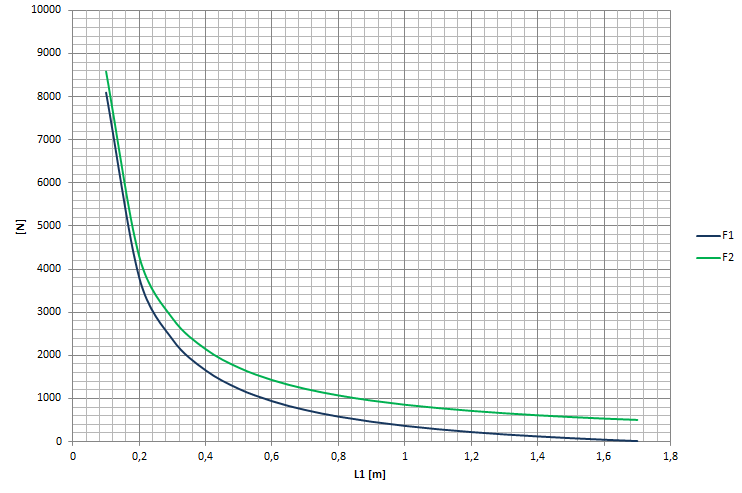
\includegraphics[width=1.0\textwidth]{images/Bilden_2}
\end{center}
\caption{$F_1$ og $F_2$ som en funksjon av $L_1$}
\label{fig:Krefter}
\end{figure}

Setter minste verdi av $L_1$ lik 0.5 m. Vil da få opplagerkrefter på $F_1$ lik 1230 N og $F_2$ lik 1720 N. Dette er de største opplagerkreftene som kan oppstå, og det er disse verdiene som brukes videre i styrkeberegningene.


